\documentclass[accentcolor=tud7b,noresetcounter]{tudbeamer}

\usepackage[ngerman]{babel}
\usepackage[utf8]{inputenc}
\usepackage[T1]{fontenc}

% footmisc behebt u.a. Probleme mit Fu?noten in Abschnittstiteln
\usepackage[stable]{footmisc}

% Einbinden von Grafiken erm?glichen
\usepackage{graphicx}

% Paket xtab erm?glicht Umbrechen von langen Tabellen
\usepackage{xtab}
\usepackage{tikz}

% picins erlaubt das Umflie?en von Abbildungen durch Text
% Untenstehendes renewcommand behebt den picins-bug, dass Abbildungen
% nicht im Abbildungsverzeichnis auftauchen
%\usepackage{picins}
\makeatletter
%\renewcommand\piccaption{\@dblarg{\@piccaption}}
\makeatother

\usepackage{verbatim}

% Paket setspace erlaubt Umschalten auf 1.5fachen Zeilenabstand
\usepackage{setspace}

\usepackage{hyperref}
\usepackage{listings}
\usepackage{amssymb}
\usepackage{newclude}
\usepackage{multirow}
\usepackage{array}
\usepackage{tabularx}
\usepackage{hyperref} 
\usepackage{graphicx}
\usepackage{pgfplots}
\usepackage{csvsimple}
\usepackage{wrapfig}
%Erm?glicht Hyperlinks zwischen Textstellen und zu externen Dokumenten
%% breaklinks=true/false: Gibt an, ob Links umgebrochen werden d?rfen.
%% linktocpage=true/false: im Inhaltsverzeichnis sind nur die Seitenzahlen
%% links, nicht der Text
%% colorlinks=true/false: Links werden eingef?rbt (Farben werden mit
%% linkcolor, anchorcolor \dots festgelegt)
%% linkcolor=Farbe: Farbe des verlinkten Textes, Dokument-interne Links
%% citecolor=Farbe: Farbe des verlinkten Textes, Links zum
%% Literaturverzeichnis
%% filecolor=Farbe: Farbe des verlinkten Textes, Links auf lokale Dateien
%% urlcolor=Farbe: Farbe des verlinkten Textes, externe URLs
%% frenchlinks=true/false: Links werden als smallcaps, anstatt farbig
%% dargestellt.
%% breaklinks=true/false: Gibt an, ob Links umgebrochen werden d?rfen.
\hypersetup{%
  linktocpage=true,
  breaklinks=true,
  colorlinks=true,
  citecolor=black,
  urlcolor=black,
  linkcolor=black,
  pdfpagemode=UseThumbs,
  pdftitle=Übung 2 - Webmining,
  pdfauthor=Ingo Adrian und Steffen Pegenau,
  pdfsubject=Webmining,
  %pdfkeywords=xy
}

\tikzset{
  every overlay node/.style={
    draw,
    anchor=north west,
  },
}
\def\tikzoverlay{%
   \tikz[baseline,overlay]\node[every overlay node]
}%


\lstset{ %
  %backgroundcolor=\color{white},   % choose the background color; you must add 
%\usepackage{color} or \usepackage{xcolor}
  %basicstyle=\footnotesize,        % the size of the fonts that are used for 
					%the code
  %breakatwhitespace=false,         % sets if automatic breaks should only 
%happen at whitespace
  breaklines=true,                 % sets automatic line breaking
  %captionpos=b,                    % sets the caption-position to bottom
  commentstyle=\bf,    % comment style
  %deletekeywords={...},            % if you want to delete keywords from the 
%given language
  %escapeinside={\%*}{*)},          % if you want to add LaTeX within your code
  %extendedchars=true,              % lets you use non-ASCII characters; for 
%8-bits encodings only, does not work with UTF-8
  frame=single,                    % adds a frame around the code
  %keepspaces=true,                 % keeps spaces in text, useful for keeping 
%indentation of code (possibly needs columns=flexible)
  %keywordstyle=\color{blue},       % keyword style
  language=html,                 % the language of the code
  %otherkeywords={*,...},            % if you want to add more keywords to the 
%set
  numbers=left,                    % where to put the line-numbers; possible 
%values are (none, left, right)
  %numbersep=5pt,                   % how far the line-numbers are from the code
  %numberstyle=\tiny\color{mygray}, % the style that is used for the 
%line-numbers
  %rulecolor=\color{black},         % if not set, the frame-color may be changed 
%on line-breaks within not-black text (e.g. comments (green here))
  %showspaces=false,                % show spaces everywhere adding particular 
%underscores; it overrides 'showstringspaces'
  %showstringspaces=false,          % underline spaces within strings only
  %showtabs=false,                  % show tabs within strings adding particular 
%underscores
  %stepnumber=2,                    % the step between two line-numbers. If it's 
%1, each line will be numbered
  %stringstyle=\color{mymauve},     % string literal style
  tabsize=4,                       % sets default tabsize to 2 spaces
  %title=\lstname                   % show the filename of files included with 
%\lstinputlisting; also try caption instead of title
}

% bibtex
%\usepackage[backend=biblatex]{biblatex}

%\bibliography{refs}
%\addbibresource{refs.bib}

%%%%%%%%%%%%%%%%%%%%%%%%%%%%%%%%%%%%%%%%%%%%%%%%%%%%%%%%%%%%%%%%%%%%%%%%%%%%%%%%%%%%%%

\title%[Klima \& Geographie] % (optional, only for long titles)
{Web Mining: Übung 3}
\subtitle{Lösungsvorschlag}

\author[Ingo Adrian und Steffen Pegenau]{}
\institute[Fachbereich Informatik]{}
\date[\today]
%%%%%%%%%%%%%%%%%%%%%%%%%%%%%%%%%%%%%%%%%%%%%%%%%%%%%%%%%%%%%%%%%%%%%%%%%%%%%%%%%%%%%

\pgfplotsset{compat=1.12}

\begin{document}
  
  \begin{titleframe}
  \end{titleframe}
  
  \begin{frame}
  \frametitle{Aufgabe 1:\\ Einteilung der Testdaten}
  \begin{itemize}
    \item Verwendeter Testdatensatz: Co-training Experiments for COLT 98\\
    \url{http://www.cs.cmu.edu/afs/cs.cmu.edu/project/theo-51/www/co-training/data/}
    \item Testdaten sind in Unterordnern sortiert:\\
    	  Art/Kategorie/VolleURL
   \item Art kann "`fulltext"' oder "`inlinks"'
   \item "`fulltext"': HTML-Dateien
   \item "`inlinks"': Link-Text(e), die auf die Seiten verwiesen haben. \\
	Beispiel: \texttt{<a href=VolleURL>Link-Text</a>}
   \item Zur einfacheren Verarbeitung soll die Ordnerhierarchie entfallen und
   	die Informationen in den Dateinamen übernommen werden.
  \end{itemize}
  \end{frame}
  
  \begin{frame}
  \frametitle{Aufgabe 1:\\ BASH: Neusortierung/Entfernung der Hierarchie \\ Teil 1: Die dunklen Zeichen }
  \begin{itemize}
    \item Mit einem Bash-Skript soll die Hierarchie flach gezogen werden
    \item Das Namensschema der Dateien soll lauten:\\
    $\text{fulltext|inlinks}\underbrace{-----}_{\text{Trenner}}\text{Kategorie}\underbrace{-----}_{\text{Trenner}}\text{VolleURL}$
    \item Die URL soll dabei außerdem angepasst werden:
	\begin{itemize}
		\item Doppelpunkte werden entfernt, weil sich Windows daran stört
		\item \texttt{http://www.} wird ersetzt, um die URLs zu verkürzen. Windows stört sich auch an langen Dateipfaden
	\end{itemize}
    \item Am Ende sehen die Dateinamen so aus: \\
    $\underbrace{fulltext}_{Art}--\underbrace{course}_{Kategorie}--\underbrace{BEG}_{http...}--\text{cs.washington.edu\^{}education\^{}courses\^{}431\^{}}$
    \item Vorteil des Ersetzens gegenüber dem Wegwerfen einzelner Zeichen/Abschnitte: Es gehen keine Informationen verloren. Bei Bedarf kann der gesamte Link wiederhergestellt werden.
  \end{itemize}
  \end{frame}
 
	\begin{frame}
		\frametitle{Aufgabe 1: \\ BASH: Neusortierung/Entfernung der Hierarchie \\ Teil 2: Angriff der Kategorisierung}
		\begin{itemize}
			\item Die Daten müssen nun noch in Test- und Trainingsdaten eingeteilt werden
			\item Das Skript wirft für jede Datei die Münze und dokumentiert das Ergebnis ebenfalls im Dateinamen
			\item Beispiel: \\
			\texttt{test----fulltext----course----BEG----cs.wisc.edu\^{}\~{}dyer\^{}cs766.html}
			\item Das Ergebnis der Verteilung scheint zufällig und damit brauchbar: \\
			\begin{tabular}{|l|r|r||r|}
				\hline
& Training	& Test	& 	Summe \\
\hline
course	& 	233	& 	227	& 	460	\\
non-course	& 	802	& 	840	& 	1642	\\
\hline
\hline
Summe	& 	1035	& 	1067	& 2102\\
				\hline
			\end{tabular}
			\item Mit dem im weiteren Verlauf verwendeten libsvm lassen sich die Daten zwar einfacher und eleganter in Trainings- und Testdaten einteilen, aber da es nun mal in der Aufgabenstellung stand ...


		\end{itemize}

	\end{frame}
	
	%%%%%%%%%%%%%%%%%%%%%%%%%%%%%%%%%%%%%%%%%%%%%%%%%%%%%%%%%%%%%%%%%%%%%%%%%%%%%%%%%%%%%%%%%%
	% Aufgabe 02
	
	\begin{frame}
		\frametitle{Aufgabe 2: Aufbereitung der Daten\\Dokument zu Wort-Liste\\Beispieldokument}
		\begin{center}
			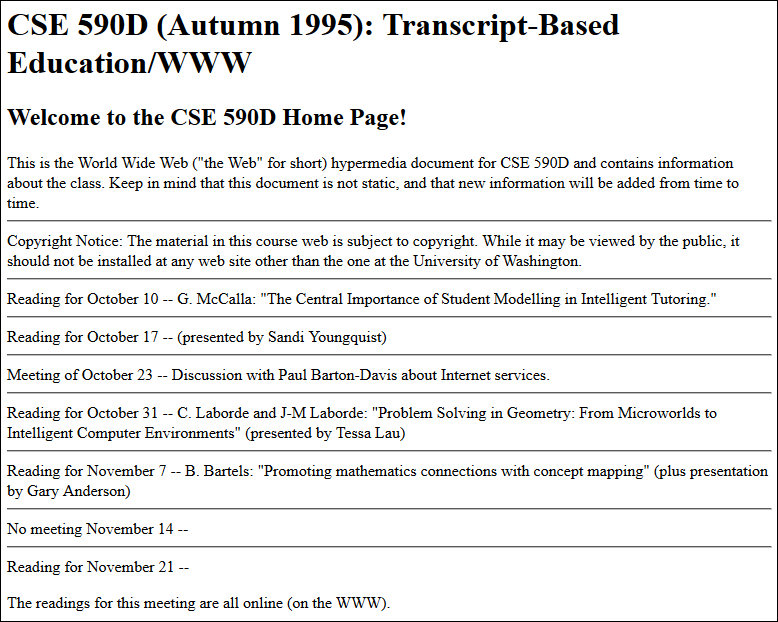
\includegraphics[height=180pt]{img/sample2}
		\end{center}
	\end{frame}
	
	\begin{frame}
		\frametitle{Aufgabe 2: Aufbereitung der Daten\\Dokument zu Wort-Liste\\Reduzierung der Wörter}
		\begin{itemize}
			\item Text aus dem html-Body wird in Kleinbuchstaben transformiert und an Leerstellen in einzelne Wörter unterteilt
			\item Emailadressen und URLs, die mit \texttt{http[s]://} beginnen, werden entfernt
			\item Wörter, die auf Satzzeichen, Klammern, Anführungszeichen etc. enden, werden um dieses reduziert
			\item Ebenso Wörter, die mit Klammern, Anführungszeichen o.ä. beginnen
		\end{itemize}
		\textbf{Beispiel:}\\
		\texttt{(autumn} wird zu \texttt{autumn}\\
		\texttt{page!} wird zu \texttt{page}\\
		\texttt{public,} wird zu \texttt{public}\\
		\texttt{1995):} wird zu \texttt{1995}
	\end{frame}
	
	\begin{frame}
		\frametitle{Aufgabe 2: Aufbereitung der Daten\\Stopwords und Stemming}
		\begin{itemize}
			\item Die verbliebenen Wörter werden um Stopwords\footnotetext{baba} aus einer Liste reduziert
			\begin{itemize}
				\item Vorher: 381 Wörter
				\item Nachher: 231 Wörter
			\end{itemize}
			%\item Quelle der Stopwords: \texttt{http://www.nltk.org/nltk\_data/packages/corpora/stopwords.zip}
			\item Anschließendes Stemming der Wörter mit dem Porter Stemmer\\\texttt{https://tartarus.org/martin/PorterStemmer/}
			\begin{itemize}
				\item Von den 231 Wörtern verbleiben 160 verschiedene Wortstämme
			\end{itemize}
		\end{itemize}
		\textbf{Stemming-Beispiele:}\\
			\texttt{welcome} $\rightarrow$ \texttt{welcom}\\
			\texttt{contains} $\rightarrow$ \texttt{contain}\\
			\texttt{information} $\rightarrow$ \texttt{inform}\\
			\texttt{added} $\rightarrow$ \texttt{ad}\\
			
	\end{frame}
	
	\begin{frame}
		\frametitle{Aufgabe 2: Aufbereitung der Daten\\TF-IDF-Vektor}
		\begin{itemize}
			\item normalisierte TF des Terms t in Dokument d: $\operatorname{tf}(t,d) = \frac{f(t, d)}{\max\{f(w, d):w \in d\}}$
			\item inv. Document Frequency: $\operatorname{idf}_i = \log \frac{N}{n_i}$
			\item Gewichtung der einzelnen Wörter: $w_{i,j} = \operatorname{tf}_{i,j} \cdot \operatorname{idf}_i$
		\end{itemize}
		
		\textbf{Werte der Beispieldatei im Trainingsset:}\\
		\texttt{TF-IDF-Vektor:}\\
		\texttt{\{'cse': 0.7920241942426215, '590d': 1.2435691877385933, 'home': 0.04761829630391385, 'page': 0.029480629516760913, 'autumn': 0.502504280189381, '1995': 0.1530192780213716, ...\}}
	\end{frame}
	
	\begin{frame}
		\frametitle{Aufgabe 2: Aufbereitung der Daten\\Sparse-Darstellung}
		\begin{itemize}
			\item Die 10 häufigsten Wörter nach Dokumenthäufigkeit:\\
			\texttt{$\lbrack$('page', 234), ('comput', 234), ('home', 198), ('scienc', 197), ('univers', 189), ('depart', 149), ('1996', 133), ('inform', 128), ('research', 128), ('system', 127)$\rbrack$}
			
			\item Sparse-Format:\\
			\texttt{+1 1:0.029480629516760913 2:0.014740314758380457 3:0.04761829630391385 5:0.026334571412992794 8:0.1424731521859943}
			\item Bedeutung:
			\begin{itemize}
 				\item \texttt{page} hat eine TF-IDF-Gewichtung von \texttt{0.029480629516760913}
 				\item \texttt{comput} hat eine TF-IDF-Gewichtung von \texttt{0.014740314758380457}
 				\item \texttt{home} hat eine TF-IDF-Gewichtung von \texttt{0.04761829630391385}
 				\item \texttt{scienc} ist nicht im Dokument vorhanden
 				\item \texttt{univers} hat eine TF-IDF-Gewichtung von \texttt{0.026334571412992794}
 				\item usw.
			\end{itemize}
		\end{itemize}
	\end{frame}
	
	\begin{frame}
		\frametitle{Aufgabe 3:\\ Analyse der erhobenen Daten\\ Teil 1: Statistische Analyse -- Konfusionsmatrix}
		\begin{itemize}
			\item Trainingsdaten: 151, Testdaten: 152
			\item Konfusionsmatrix: \\
			\begin{tabular}{|l|l|c|c||c|}
		\hline
			& & \multicolumn{2}{c|}{Vorhersage} & \\
			\hline
			& & course & non-course & Summe \\
			\hline
		\multirow{2}{*}{Kategorie} & course (+1) & 20 & 21 & 41\\
		\cline{2-5}
		& non-course (-1) & 8 & 103 & 111\\
		\hline
		& Summe & 28 & 124 & 152 \\
		\hline
		\end{tabular}
			\item Accuracy: $A = \frac{TP + TN}{N} = \frac{20+103}{152} \approx 80,92\%$
			\item Trainingszeit: 0,027884 Sekunden (-t 0 -c 50, 284 Iterationen)\\
				Testzeit: 0,02458 Sekunden
		\end{itemize}

		

	\end{frame}
	
	\newcommand{\plotOf}[3]{
 \resizebox {0.9\columnwidth} {!} {
	  \begin{tikzpicture}
	  
	    \begin{axis}[
	    axis lines=middle,
	    axis line style={->},
	    x label style={at={(axis description cs:0.5,-0.1)},anchor=north},
	    y label style={at={(axis description cs:-0.1,.5)},rotate=90,anchor=south},
	    xlabel={#1},
	    ylabel={#2},
	    %ymin=-1,
	    %ymax=110
	    ]
	    \addplot table [x=features, y=#3,col sep=semicolon]
	    %,col sep=semicolon
	    {../Aufg03/3.3result.csv};
	  \end{axis}
	  \end{tikzpicture}
	  }
}
	
	\begin{frame}
		\frametitle{Aufgabe 3:\\ Analyse der erhobenen Daten\\ Teil 1: Statistische Analyse -- Baseline}
		\begin{itemize}
			\item Baseline: Tippt immer auf die am häufigsten vorkommende Kategorie
			\item Insgesamt sind 231 von 303 Datensätzen non-course (-1) \\
			      Ermittelt mit \texttt{cat data.txt | grep '-1' | wc -l}
			\item In den Trainingsdaten sind 231 - 111 = 120 von 152 Datensätzen non-course
			\item Die Baseline Konfusionsmatrix sieht also so aus: \\
			\begin{tabular}{|l|l|c|c||c|}
		\hline
			& & \multicolumn{2}{c|}{Vorhersage} & \\
			\hline
			& & course & non-course & Summe \\
			\hline
		\multirow{2}{*}{Kategorie} & course (+1) & 0 & 32 & 32 \\
		\cline{2-5}
		& non-course (-1) & 0  & 120 & 120\\
		\hline
		& Summe & 0 & 152 & 152 \\
		\hline
		\end{tabular}
			\item Accuracy: $A = \frac{TP + TN}{N} = \frac{120}{152} \approx 78,95\%$
			\item Das trainierte Modell ist mit 80,92\% nur wenig besser, was am hohen Anteil von non-course Datensätzen liegt
		\end{itemize}
	\end{frame}
	
	\begin{frame}
	  \frametitle{Aufgabe 3.3:\\ Variation der Feature-Anzahl\\ Genauigkeit}
	    
	  %\begin{minipage}[\textheight]{\textwidth}
	    \begin{columns}[T]%T
	    \begin{column}{0.3\textwidth}
	    \begin{itemize}[] %<+->
	    \item Accuracy fällt zu\-nächst stark ab, nähert sich dann $\approx72\%$ an
	    \item Sinnvoll ist also entweder die Betrachtung von weniger als $\approx50$ Features (danach fällt Genauigkeit ab)
	    \item ...oder $\approx600$, weil danach die Genauigkeit nicht wesentlich steigt
	    \end{itemize}
	    \end{column}
	    \begin{column}{0.7\textwidth}
	    \plotOf{Anzahl Features}{Accuracy in \%}{accuracy} 
	    \end{column}
	    \end{columns}
	    %\end{minipage}
	   
  
	\end{frame}
	
	\begin{frame}
	  \frametitle{Aufgabe 3.3:\\ Variation der Feature-Anzahl\\ Trainingsdauer}
	  \begin{columns}[T]%T
	    \begin{column}{0.4\textwidth}
	    \begin{itemize}[] %<+->
	    \item Trainingsdauer steigt von Ausreißern abgesehen etwa linear an
	    \item Selbst mit vielen Features beträgt die Dauer jedoch weniger als eine Sekunde
	    \item $\rightarrow$ Trainingsdauer eher nicht maßgeblich für Wahl der Anzahl
	    \end{itemize}
	    \end{column}
	    \begin{column}{0.6\textwidth}
	    \plotOf{Anzahl Features}{Trainingsdauer in Sekunden}{timeTraining} 
	    \end{column}
	    \end{columns}
	  
	\end{frame}
	
	\begin{frame}
	  \frametitle{Aufgabe 3.3:\\ Variation der Feature-Anzahl\\ Testdauer}
	  \begin{columns}[T]%T
	    \begin{column}{0.4\textwidth}
	    \begin{itemize}[] %<+->
	    \item Die Testdauer ist nicht linear
	    \item Abnehmende Grenzrate
	    \item Auch bei vielen Features weit unter einer Sekunde
	    \end{itemize}
	    \end{column}
	    \begin{column}{0.6\textwidth}
	    \plotOf{Anzahl Features}{Testdauer in Sekunden}{timeTesting}
	    \end{column}
	    \end{columns}
	  
	\end{frame}
	




% etc
\end{document}